% This example requires PGF >= 1.09 and only works wit PDFTeX
% You have to compile document twice to get correct placement of nodes.
\documentclass{beamer} %
\usepackage{tikz}
\usepackage{verbatim}

\usetikzlibrary{arrows,shapes,backgrounds}

\begin{document}

\begin{comment}
:Title: Connecting text and graphics
:Tags: Remember picture, Beamer, Overlays

With PGF 1.09 and later, it is possible to draw paths between nodes across
different pictures. In this example I have used this feature to connect text with
coordinate nodes placed on a picture. The picture is loaded from an external file
A background grid is used to make it easier to place the coordinates manually.

**Note.** This only works with PDF(La)TeX, and you have to run PDFTeX twice.

Source: Inspired by a post_ to the latex-beamer-users list. The Daniell's pile 
illustration_ is made by Augustin E. Bolzan.

.. _post: http://sourceforge.net/mailarchive/message.php?msg_name=200704100122.41993.cedric.Laczny%40gmx.de
.. _illustration: http://www.fauskes.net/pgftikzexamples/daniells-pile/

\end{comment}


% For every picture that defines or uses external nodes, you'll have to
% apply the 'remember picture' style. To avoid some typing, we'll apply
% the style to all pictures.
\tikzstyle{every picture}+=[remember picture]
\tikzstyle{na} = [baseline=-.5ex]

\begin{frame}

\frametitle{Daniell's pile, saline bridge version}

\begin{columns}
    \begin{column}{0.4\paperwidth}
        % define source coordinates
        \begin{itemize}
            \item Anode \tikz[na] \coordinate (s-anode);
            \item Cathode \tikz[na] \coordinate (s-cathode);
            \item Saline bridge \tikz[na] \coordinate (s-bridge);
        \end{itemize}
        
    \end{column}
    \begin{column}{0.45\paperwidth}
        % Use a background grid to make it easier to find coordinates
        % When the coordinates have been found, remove the 
        % 'show background grid' option. 
        \tikzstyle{background grid}=[draw, black!50,step=.5cm]
        \begin{tikzpicture}[show background grid]
            % Put the graphic inside a node. This makes it easy to place the
            % graphic and to draw on top of it. 
            % The above right option is used to place the lower left corner
            % of the image at the (0,0) coordinate. 
            \node [inner sep=0pt,above right] 
                {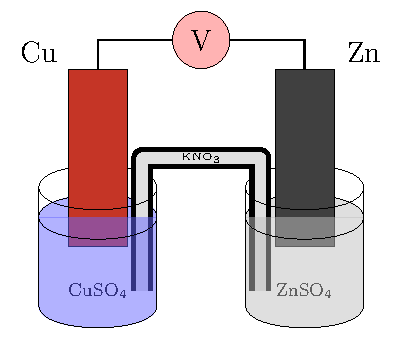
\includegraphics[width=4cm]{img/daniells-pile}};
            % show origin
            \fill (0,0) circle (2pt);
            % define destination coordinates
            \path (0.7,2) coordinate (cathode)
                  (2,1.8) coordinate (bridge)
                  (2.75,2.5) coordinate (anode);
        \end{tikzpicture}
    \end{column}
\end{columns}

% define overlays
% Note the use of the overlay option. This is required when 
% you want to access nodes in different pictures.
\begin{tikzpicture}[overlay]
        \path[->,red,thick] (s-anode) edge [bend left] (anode);
        \path[->,blue,thick] (s-cathode) edge [bend left] (cathode);
        \path[->,red,thick] (s-bridge) edge [out=0, in=-90] (bridge);
\end{tikzpicture}

\end{frame}

\end{document}